\documentclass[10pt]{article}

\usepackage[skip=7pt plus1pt, indent=0pt]{parskip}
\usepackage{hyperref}
\usepackage[margin=0.7in]{geometry}
\usepackage{cite}
\usepackage{graphicx}
\usepackage{caption}
\usepackage{subcaption}
\usepackage{float}
\thispagestyle{empty}

\AtBeginDocument{%
  \providecommand\BibTeX{{%
    Bib\TeX}}}

\newcommand{\tall}{\phantom{\large PQq}}
\thispagestyle{empty}

\begin{document}
\thispagestyle{empty}

\vspace{-2em}
\title{\huge \textsc{cmpe-258}: Hand-drawn Flowchart Recognition}
\date{}

\vspace{-2em}
\author{}
% \author{Mu Chen, Roger Kuo, Hardy Leung, Jasmine Wang}

\maketitle

\vspace{-5em}

\begin{figure}[h]
\centering
\begin{subfigure}{0.30\columnwidth}
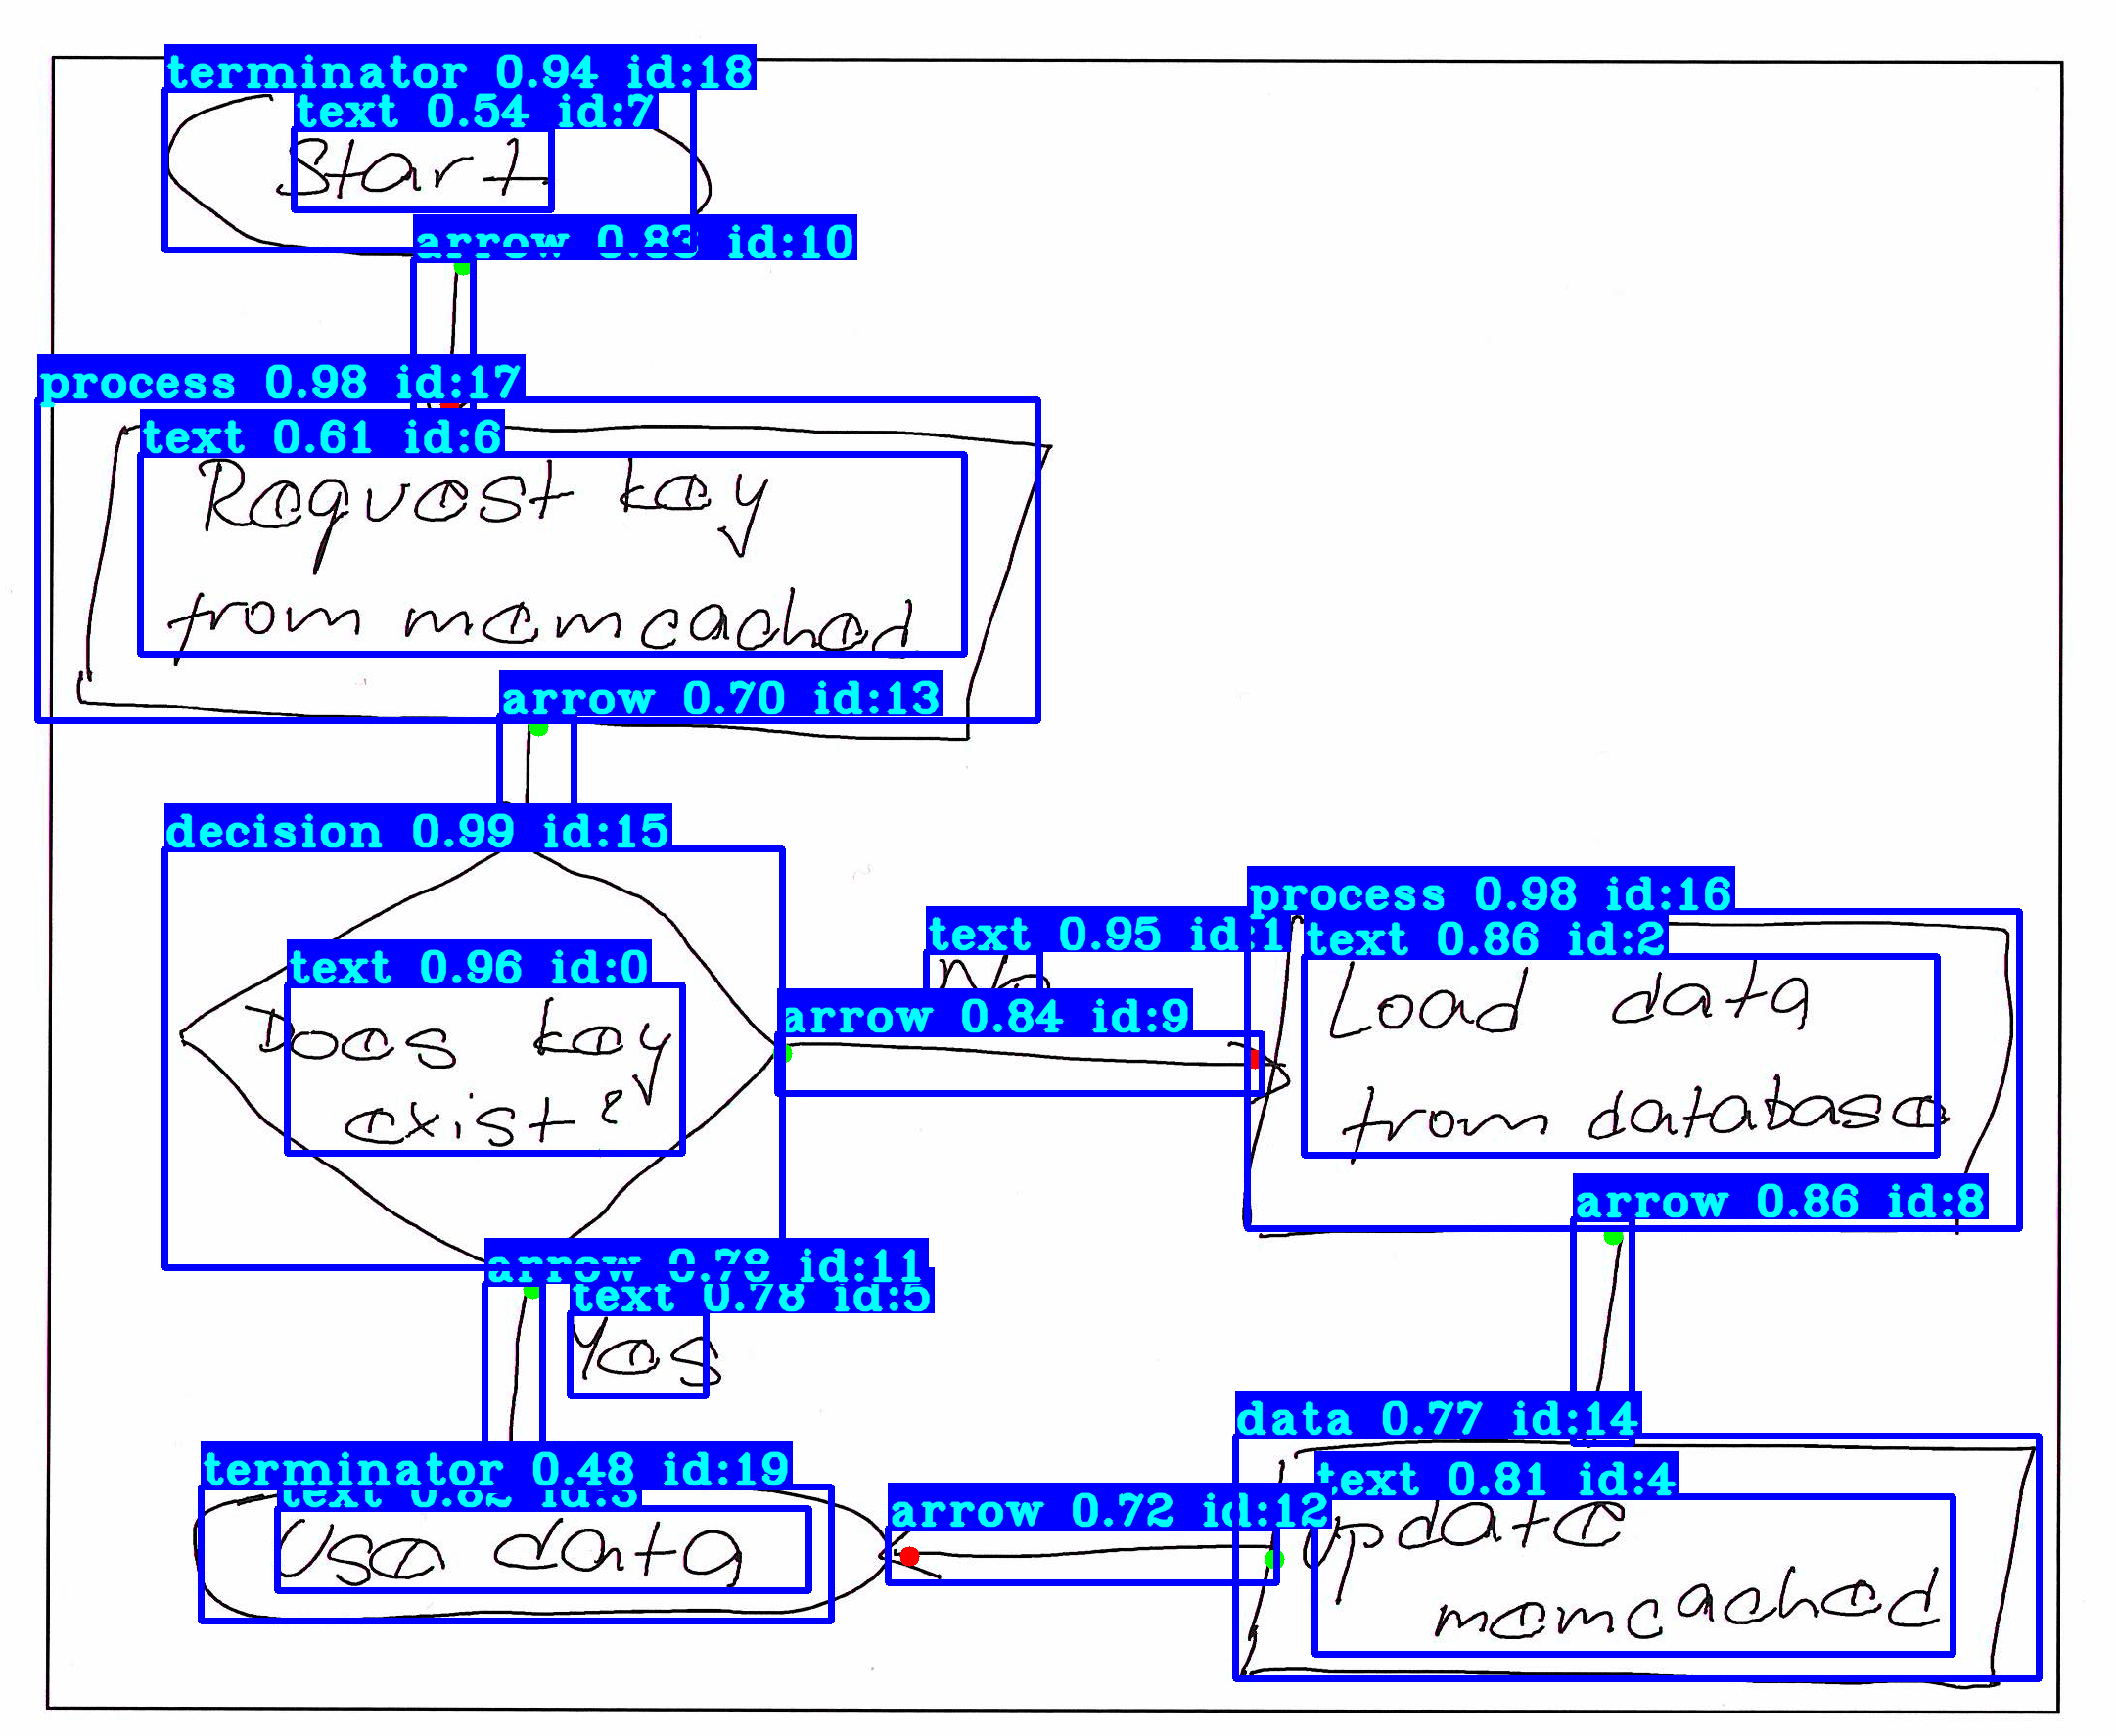
\includegraphics[width=\columnwidth]{sample.png}
\end{subfigure}
\begin{subfigure}{0.30\columnwidth}
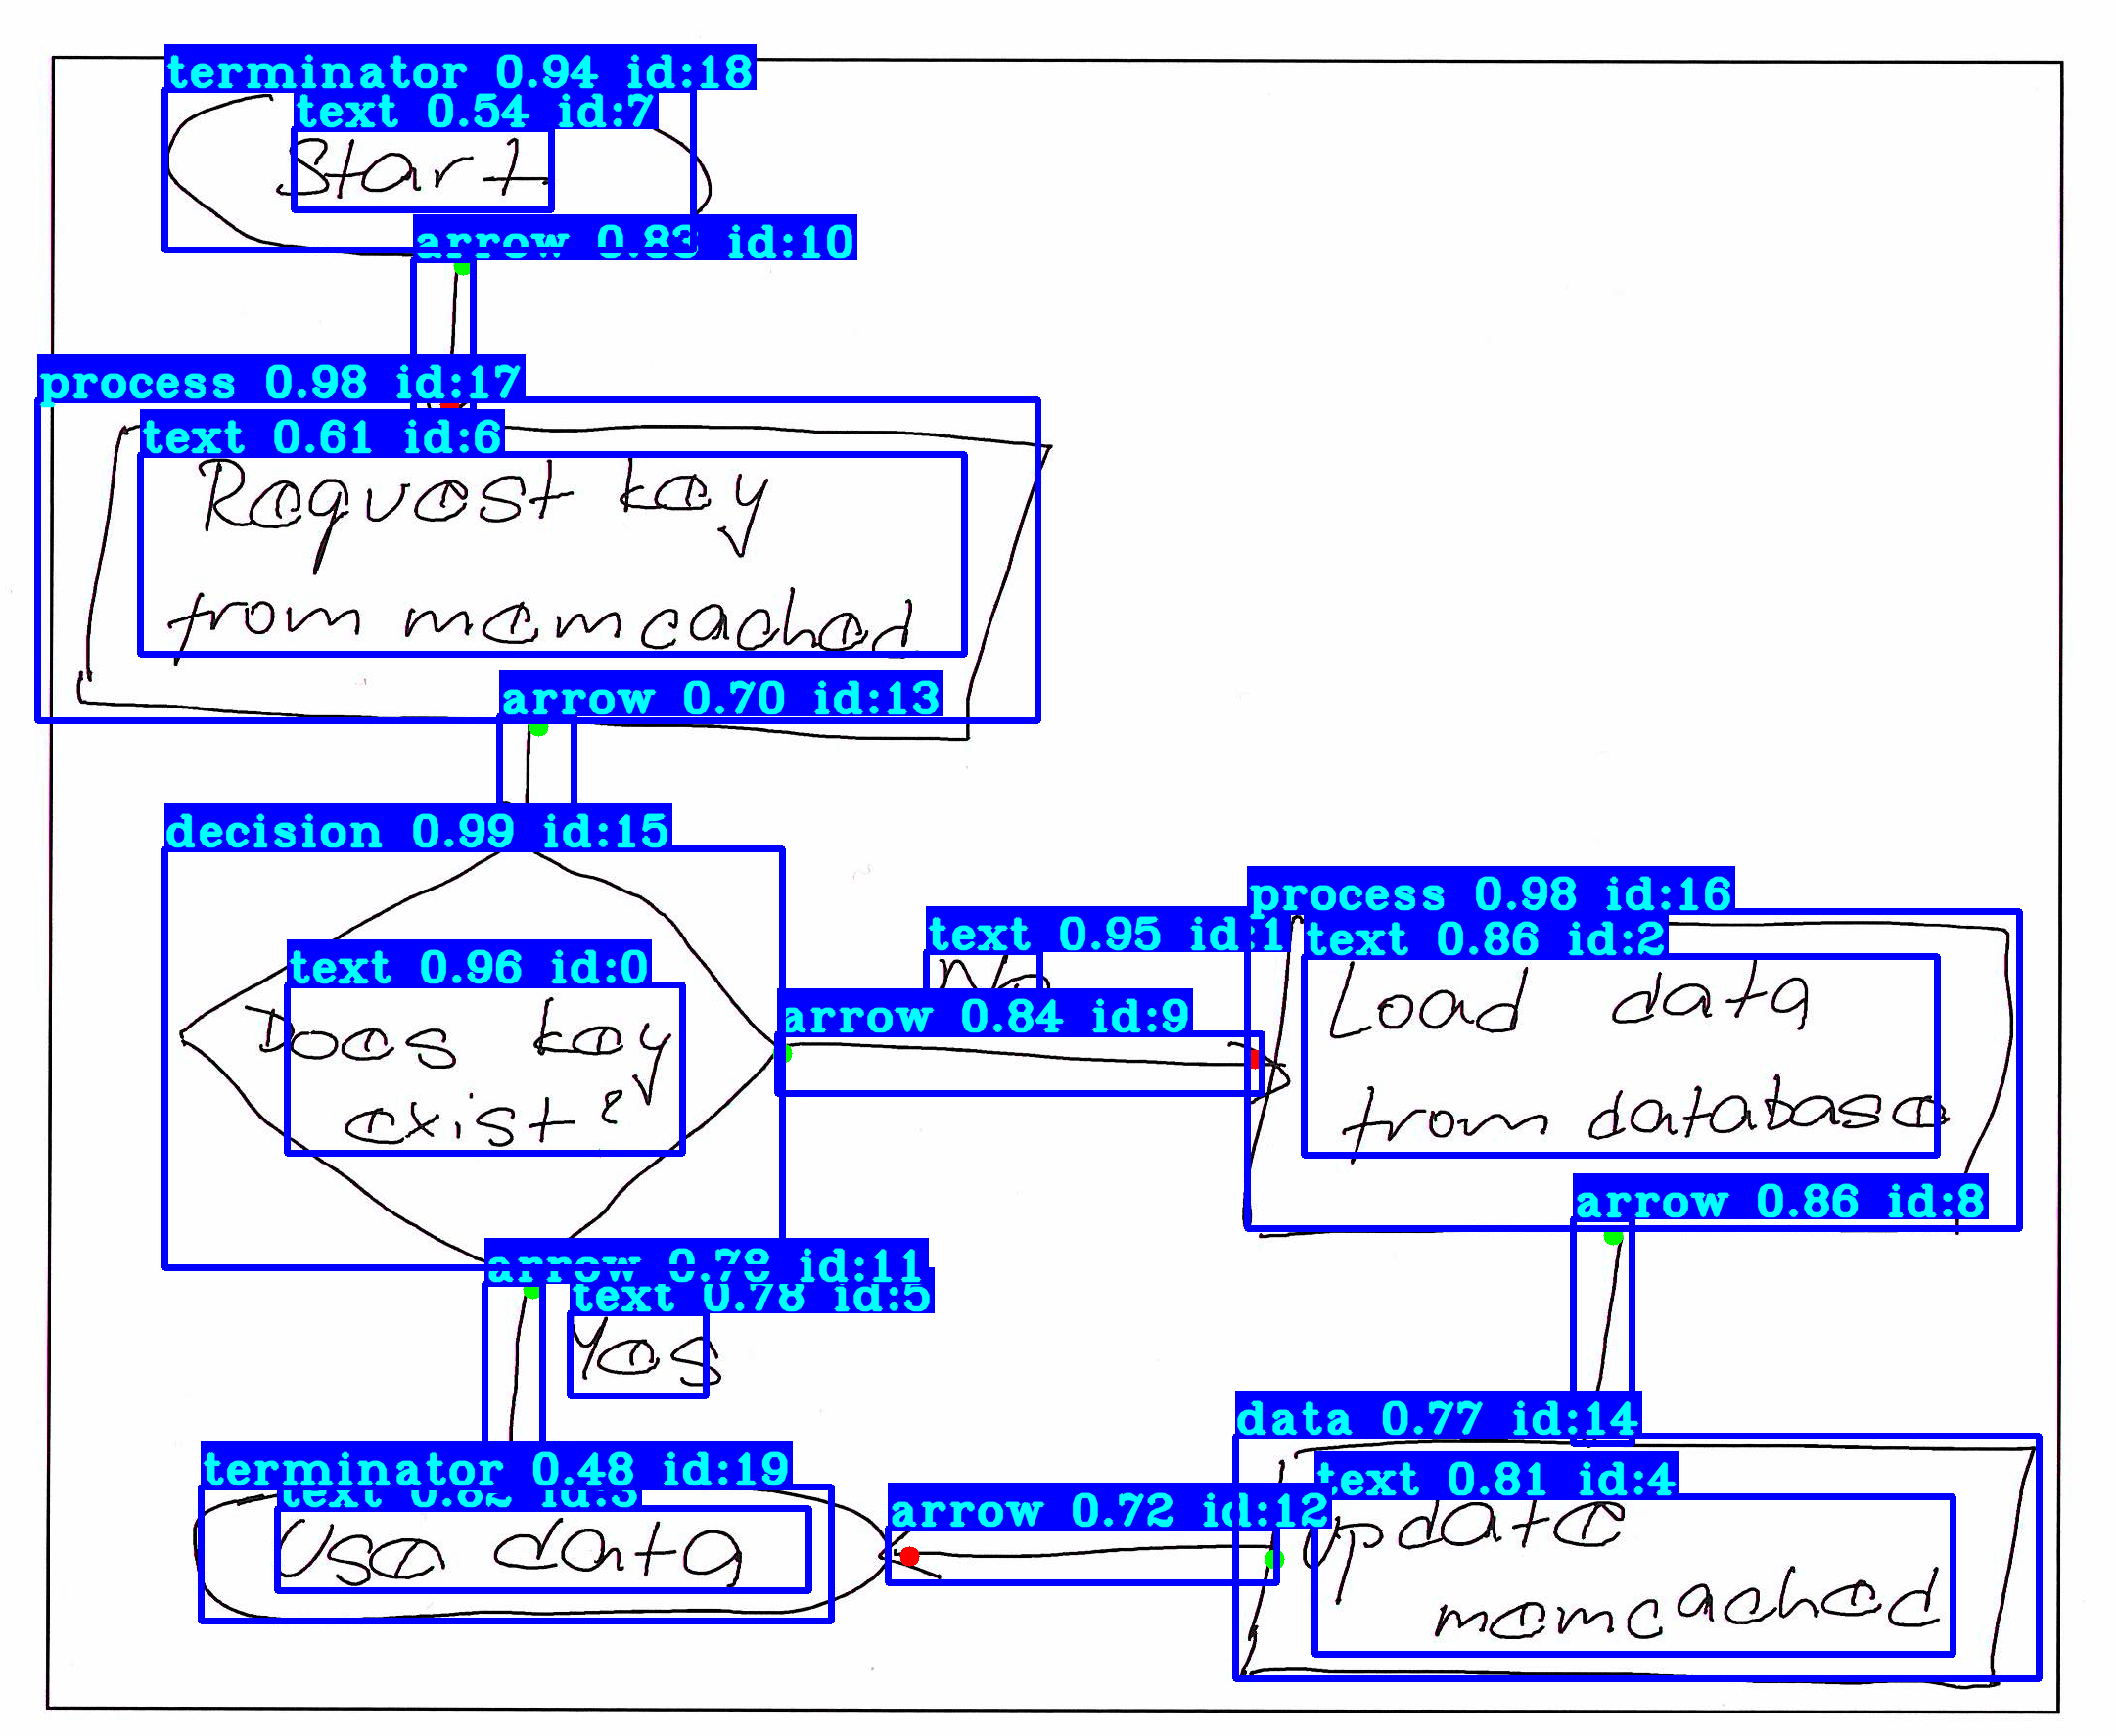
\includegraphics[width=\columnwidth]{sample.png}
\end{subfigure}
\begin{subfigure}{0.30\columnwidth}
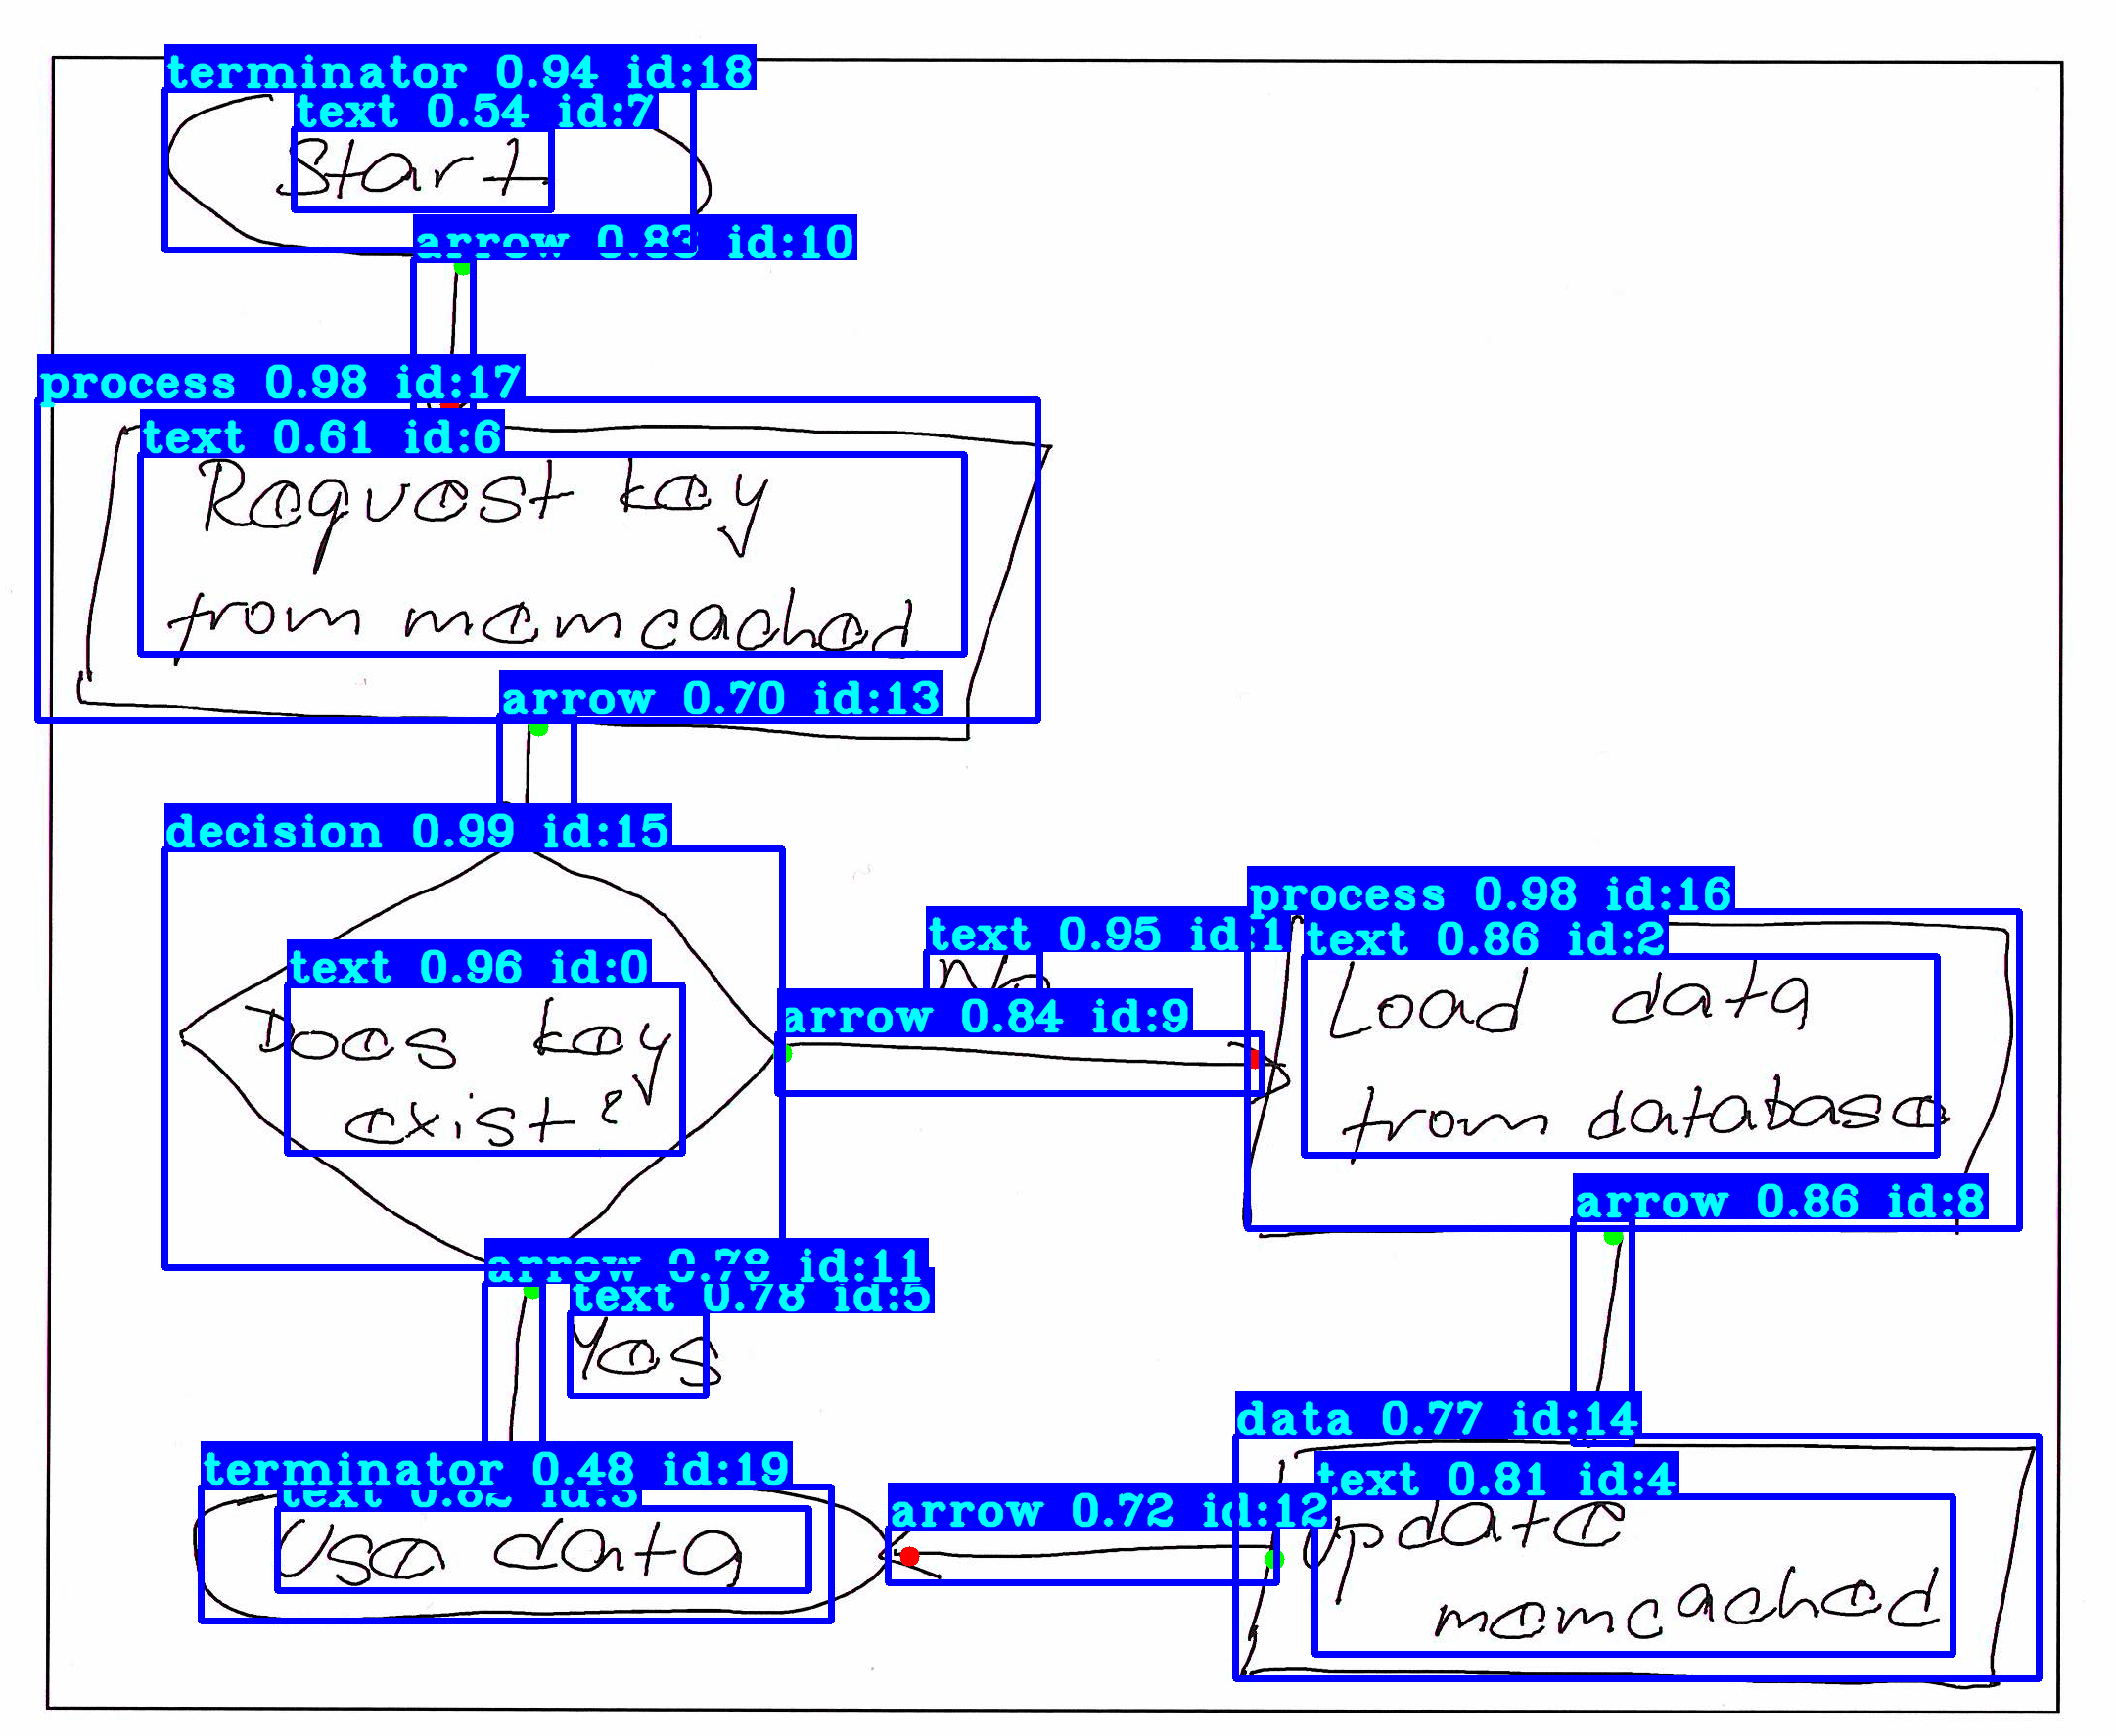
\includegraphics[width=\columnwidth]{sample.png}
\end{subfigure}
\end{figure}

Flowcharts are incredibly versatile and flexible tools, often the most
succinct way to summarize or visualize concepts such as workflow and
relationships.
While all productivity softwares support the creation of flowcharts through
drawing primatives such as circles, blocks, and arrows, the creation
process is often awkward and unwieldy.  Many people avoid flowcharts due to such
difficulty, as well as the inevitable discrepancy between what was intended and how it
turns out. As such, 
the objective of our project is to apply deep-learning techniques to develop a
hand-drawn flowchart recognition system
that accurately translates user's intent to actual rendering of flowcharts in
productivity applications.

The key ingredient of our flowchart recognition system is the
\textsc{yolo-v4} engine custom trained to detect flowchart objects.
We then analyze these elements and extract connectivity and
symbolic relationships between them, and perform \textsc{ocr} to convert
handwritings to actual English words. The result is a symbolic flowchart that fully
captures the positional, relational, and textual intents, which we can then render
in a variety of dfferent ways.
In the following, we describe our algorithm in more technical details.

\begin{itemize}

\item Our model is a custom \textsc{yolo-v4} deep neural network
trained to detect seven custom classes, each corresponding to
a key flowchart concept: \texttt{text}, \texttt{arrow},
\texttt{data} (parallelograms), \texttt{decision} (diamonds), \texttt{process} (straight
or rounded rectangles), \texttt{terminator}, and \texttt{connection} (input/output).

\item We used a training dataset with $600+$ high-quality annotated flowchart
images, with custom scripts to proprocess \textsc{xml}.
The training was done on Google Colab with \textsc{gpu}, taking $6+$ hours
starting with pre-trained \textsc{yolo} weights.
Our model achieved $90\%+$ mAP, with $96\%+$ accuracy on
all flowchart elements except arrows and texts.

\item We wrote post-processing code to collect the list of detected objects with a
rich set of positional and logical attributes.
Hand-writings are identified and converted to actual text using
Google's \textsc{tesseract-ocr} engine.

\item We wrote a highly accurate custom algorithm to detect arrow direction
using \textsc{openCV}, which allows us to establish the full logical relationship
between flowchart elements. Together with the shapes and text elements, we now
have a full symbol representation of the flowchart.

\item For demonstration purpose,
we recreate the flowchart in \textsc{schemDraw} as intended by
the user, doing so by following the logical order of arrows.
Our project can be easily extended to
output many other formats including \textsc{svg}, various Python drawing
formats (e.g.~Turtle and iPyCanvas), Asymptote for \LaTeX, Graphviz, and so on.

\item All in all, we utilized the following tools in the project: Python 3.8,
\textsc{openCV} 2.0, Pytorch 2.0, \textsc{yolo} scripts from PyLessons,
Google Colab (for fast \textsc{gpu}-based training),
\textsc{yolo-v4}, Google \textsc{tesseract}, and
\textsc{schemDraw}.
\end{itemize}

%\begin{center}
%\rule{0.5\textwidth}{0.05pt}
%\end{center}

%In conclusion,
%we have successfully implemented a \textsc{yolo-v4} based program to
%recognize hand-drawn flowcharts, and demonstrated the effectiveness of our
%method.
%The following summarizes our individual contributions
%(\textsc{C} = coding, \textsc{TV} =
%testing and verification,
%\textsc{P} = PPT, \textsc{ES} = executive summary. $\star$ Project Coordinator).

% \subsection*{Contributions}

\begin{table}[htbp]
\centering
\begin{tabular}{|c|c|c|c|c|c|c|c|}
\hline
Name & Major, SJSU ID & Main Responsibility & \textsc{C} &
	\textsc{T\&V} & \textsc{P} & \textsc{ES} & Overall \\
\hline
Mu Chen & SE, 014725425 & R\&D, \textsc{yolo}, \textsc{schemDraw} & $40\%$ & $40\%$ & $10\%$ & $10\%$ & $25\%$ \\
Roger Kuo & SE, 013784706 & R\&D, \textsc{yolo}, Arrow Detection & $40\%$ & $40\%$ & $10\%$ & $10\%$ & $25\%$ \\
Hardy Leung${}^\star$ & AI, 016711877 &
Proposal, Summary, Coordination & $10\%$ & $10\%$ & $10\%$ & $70\%$ & $25\%$ \\
Jasmine Wang & AI, 002805362 & Testing, Presentation & $10\%$ & $10\%$ & $70\%$ & $10\%$ & $25\%$ \\ \hline
\end{tabular}
%The following summarizes our individual contributions
\caption{\textsc{C} = coding, \textsc{TV} =
testing and verification,
\textsc{P} = PPT, \textsc{ES} = executive summary. $\star$ Project Coordinator}
\end{table}

% \bibliographystyle{acm}
% \bibliography{paper}

\end{document}
